\documentclass{beamer}
\mode<presentation>
{
  \usetheme{NYU}      % or try Darmstadt, Madrid, Warsaw,
  \usecolortheme{default} % or try albatross, beaver, crane,
  \usefonttheme{default}  % or try serif, structurebold, ...
  \setbeamertemplate{navigation symbols}{}
  \setbeamertemplate{caption}[numbered]
}
\usepackage{tikz}
\usepackage{minted}
\usepackage[greek,english]{babel}
\setbeamertemplate{blocks}[default]
\useinnertheme{rectangles}
\usepackage{hyperref}
\usepackage{graphicx}
\usepackage{amssymb}
\usepackage{algpseudocode}
\usepackage[ruled,vlined,linesnumbered]{algorithm2e}
\DeclareRobustCommand{\bbone}{\text{\usefont{U}{bbold}{m}{n}1}}
\DeclareMathOperator{\expected}{\mathbb{E}}% expected value
\usepackage{amsmath,array,xcolor}
%---------------------------------- max/min subscript commands
\DeclareMathOperator*{\argmax}{max}
\DeclareMathOperator*{\argmin}{min}
\usetikzlibrary{matrix,chains,positioning,decorations.pathreplacing,arrows}
\usetikzlibrary{positioning}
\usetikzlibrary{arrows}
\usepackage[english]{babel}
\usepackage[utf8x]{inputenc}
\title[ANNs, CNNs, and RNNs]{Artificial Neural Networks and Deep Learning}
\begin{document}
\begin{frame}
    \date{}
    \titlepage
    Daniel Mallory
    \newline
    Saint Michael's College
\end{frame}

% Uncomment these lines for an automatically generated outline.
\begin{frame}{Outline}
    \tableofcontents
\end{frame}

%---------------------------
\section{Introduction}
%---------------------------

%---------------------------

%---------------------------
\subsection{The History}
%---------------------------
\begin{frame}{Early Ideas}
    \begin{enumerate}[1.]
        \item Cybernetics: From the greek \textgreek{'κυβερνήτης'} (cybernetes) meaning 'to steer' 
        \begin{enumerate}[a.]
            \item A general formulation of the goal-oriented process; when 'steering' towards some goal, and you get off course, adjust and move back towards the goal
            \item Loop of: Trying $\rightarrow$ acting $\rightarrow$ noting difference $\rightarrow$ adjusting
            \item This 'goal oriented process' is a fundamental property of all 'intelligent' things
            \item This approach to Artificial Intelligence is more similar to the idea of 'Reinforcement Learning'.
        \end{enumerate}
        \item The Buzzword: Artificial Intelligence
        \begin{enumerate}[i.]
            \item The classic 'I, Robot' perspective (both the Asimov book and the Will Smith movie)
            \item For all intensive purposes, this doesn't exist 
        \end{enumerate}
    \end{enumerate}
\end{frame}
%---------------------------
%---------------------------
% THIS SLIDE TOO LONG 
\begin{frame}{AI Waves and Winters}
        \begin{enumerate}[1.]
            \item First Wave (1956-1974): The 'perceptron', which is the basis for modern FCNNs, was published by Frank Rosenblatt.
            \item First Winter (1974-1980): Financial setbacks combined with lack of computing power and overpromises.
            \item Second Wave (1980-1987): The classic "Backpropagation" paper was published, which is now the workhorse of modern nets. The neocognitron (Fukushima et al. 1980) and the fully backpropagated CNN (LeCun et al. 1988) papers were published.
            \item Second Winter (1987-1993): Rule-based systems don't generalize too well. Funding low, and hype dies down.
            \item Third Wave (1993-Present): Processing power caught up with computational requirements of neural nets. Large datasets and better algorithms (and faster GPUs/CUDA).
        \end{enumerate}
\end{frame}
%---------------------------
\subsection{The Strengths of ANNs}
%---------------------------

%---------------------------

%---------------------------
\begin{frame}{Why now?}
\begin{enumerate}[1.]
    \item Larger datasets give more accurate pictures (ha!) of tasks in which neural networks are applied
    \item Computing power (i.e. GPU/TPU) has increased massively, making processing power no longer a restricting bottleneck (depending on your resources)
    \item Architectures now exist that allow people to train sub-architectures of networks in parallel (i.e. on multiple GPUs and CPUs at once)
    \item People have just had better ideas; the inception of ideas like Convolutional Networks, Recurrent Networks, and algorithms to improve training time (i.e. Batch normalization, dropout)
\end{enumerate}
\end{frame}
%---------------------------

%---------------------------

%---------------------------
\begin{frame}
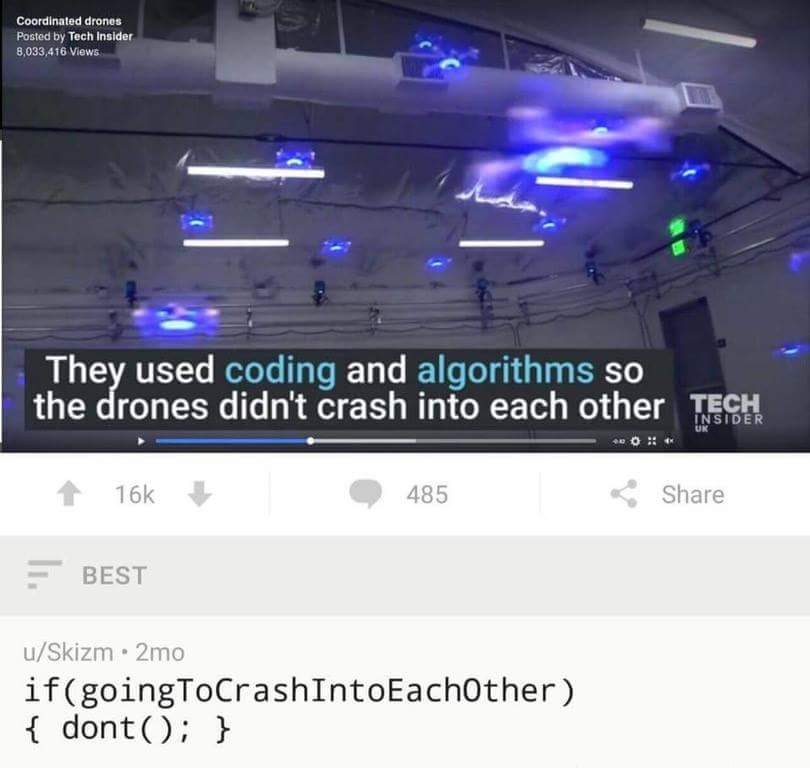
\includegraphics[width=\textwidth, height=\textheight]{images/image1.jpg}
\end{frame}
%------------------------------

%------------------------------

%------------------------------
\begin{frame}{Why Neural Networks?}
\begin{enumerate}[1.]
    \item Traditionally, computers are much faster than humans at computations
        \begin{enumerate}[a.]
            \item Complex optimization problems 
            \item Matrix multiplication
        \end{enumerate}
    \item But the reverse is also true; it is difficult to program computers to perform tasks at which humans naturally excel
        \begin{enumerate}[a.]
            \item Visual recognition / spatial organization
            \item Natural language: speech and translation
            \item Driving
        \end{enumerate}
    \item Traditional statistical and computational methods struggle to accurately capture the complexity of these tasks
        \begin{enumerate}[a.]
            \item Too many rules to encode
            \item Encoding varies too much between examples
            \item Asymptotics: more data $\rightarrow$ worse performance?
        \end{enumerate}
\end{enumerate}
% http://playground.tensorflow.org/
\end{frame}
%------------------------------------------
\begin{frame}{An example...}
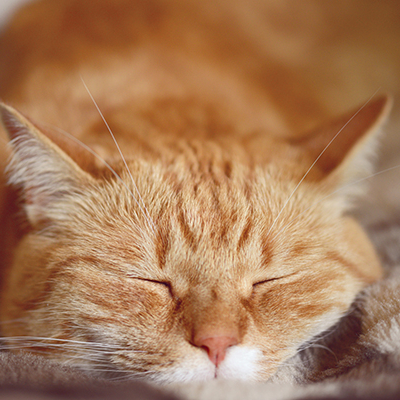
\includegraphics[width=0.5\textwidth, height=0.75\textheight]{images/img1.jpg}
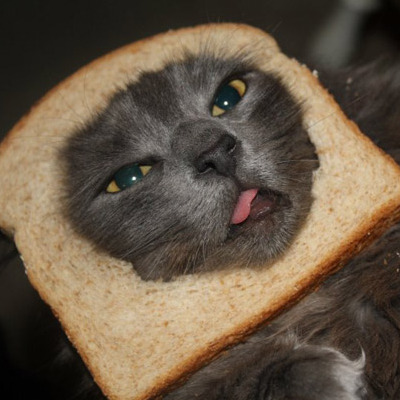
\includegraphics[width=0.5\textwidth, height=0.75\textheight]{images/img2.jpg}
\end{frame}

%-----------------------------------------
\section{Building Blocks}
%------------------------------
\subsection{The Neuron}
%------------------------------
\begin{frame}{The "Neuron"}
    \begin{tikzpicture}[
        init/.style={
        draw,
        circle,
        inner sep=2pt,
        font=\Huge,
        join = by -latex
    },
    squa/.style={
        draw,
        inner sep=2pt,
        font=\Large,
        join = by -latex
    },
        start chain=2,node distance=13mm
    ]
\node[on chain=2] 
  (x2) {$x_2$};
\node[on chain=2,join=by o-latex] 
  {$w_2$};
\node[on chain=2,init] (sigma) 
  {$\displaystyle\Sigma$};
\node[on chain=2,squa,label=above:{\parbox{2cm}{\centering Activation \\ function}}]   
  {$f$};
\node[on chain=2,label=above:Output,join=by -latex] 
  {$y$};
\begin{scope}[start chain=1]
\node[on chain=1] at (0,1.5cm) 
  (x1) {$x_1$};
\node[on chain=1,join=by o-latex] 
  (w1) {$w_1$};
\end{scope}
\begin{scope}[start chain=3]
\node[on chain=3] at (0,-1.5cm) 
  (x3) {$x_3$};
\node[on chain=3,label=below:Weights,join=by o-latex] 
  (w3) {$w_3$};
\end{scope}
\node[label=above:\parbox{2cm}{\centering Bias \\ $b$}] at (sigma|-w1) (b) {};
\draw[-latex] (w1) -- (sigma);
\draw[-latex] (w3) -- (sigma);
\draw[o-latex] (b) -- (sigma);

\draw[decorate,decoration={brace,mirror}] (x1.north west) -- node[left=10pt] {Inputs} (x3.south west);
\end{tikzpicture}
\end{frame}
%-----------------------------
\begin{frame}{A 'Deep' Neural Network}
\def\layersep{2cm}

\begin{tikzpicture}[-,draw=black!50, node distance=\layersep]
    \tikzstyle{every pin edge}=[-]
    \tikzstyle{neuron}=[circle,fill=black!25,minimum size=17pt,inner sep=0pt]
    \tikzstyle{input neuron}=[neuron, fill=red];
    \tikzstyle{output neuron}=[neuron, fill=red!50];
    \tikzstyle{hn1}=[neuron, fill=cyan];
    \tikzstyle{hn2}=[neuron, fill=orange];
    \tikzstyle{hn3}=[neuron,fill=green];
    \tikzstyle{annot} = [text width=4em, text centered]
    % Draw the input layer nodes
    \foreach \name / \y in {1,...,4}
    % This is the same as writing \foreach \name / \y in {1/1,2/2,3/3,4/4}
        \node[input neuron, pin=left:Input \y] (I-\name) at (0,-\y) {};
    % Draw the hidden layer nodes
    \foreach \name / \y in {1,...,5}
        \path[yshift=0.5cm]
            node[hn1] (H1-\name) at (\layersep,-\y cm) {};
    % Draw second hidden layer nodes
    \foreach \name / \y in {1,...,5}
        \path[yshift=0.5cm]
            node[hn2] (H2-\name) at (\layersep*2,-\y cm) {};
            
    % Draw third hidden layer nodes
    \foreach \name / \y in {1,...,5}
        \path[yshift=0.5cm]
            node[hn3] (H3-\name) at (\layersep*3,-\y cm) {};
            
    % Draw the output layer nodes
    \foreach \name / \y in {1,...,3}
        \path[yshift=-.5cm]
            node[output neuron] (O-\name) at (\layersep*4,-\y cm) {};
    % Connect every node in the input layer with every node in the
    % hidden layer 1
    \foreach \source in {1,...,4}
        \foreach \dest in {1,...,5}
            \path (I-\source) edge (H1-\dest);
    % connect every node in the hidden layer 1 with every node in the
    % hidden layer 2
    \foreach \source in {1,...,5}
    \foreach \dest in {1,...,5}
        \path (H1-\source) edge (H2-\dest);
    % connect every node in the hidden layer 2 with every node in the 
    % hidden layer 3
    \foreach \source in {1,...,5}
        \foreach \dest in {1,...,5}
            \path (H2-\source) edge (H3-\dest);
            
    % Connect every node in the hidden layer with every node in the 
    % output layer
    \foreach \source in {1,...,5}
        \foreach \dest in {1,...,3}
            \path (H3-\source) edge (O-\dest);
    % Annotate the layers
    \node[annot,above of=I-1, node distance=1.5cm] (l1) {Input layer};
    \node[annot,right of=l1] (l2) {Hidden Layer 1};
    \node[annot,right of = l2] (l3) {Hidden Layer 2};
    \node[annot, right of = l3] (l4) {Hidden Layer 3};
    \node[annot, right of = l4] {Output};
    \end{tikzpicture}
\end{frame}
%-----------------------------
\subsection{Forward/Backward Propagation}
%-----------------------------
\begin{frame}{Forward Propagation}
\small{It's sometimes helpful to think about neural networks as long chains of function compositions. Each 'layer' of the network is vector of 'functions' (or neurons) which do the following: 
\begin{enumerate}[1.]
    \item Receives the output $\textbf{x}$ of the previous layer
    \item Computes the dot product/matrix multiplication of x with its weight matrix $\textbf{W}$ and adds its bias vector $\textbf{b}$
    \item Applies its non-linearity function to obtain its 'output' vector $\textbf{x}^{'}$ which is fed into the next layer
\end{enumerate}
\centerline{From the previous example:}}
\scriptsize{
$$x^{'}=\sigma\left(
\left[\begin{array}{@{} >{\color{gray}}c >{\color{gray}}c >{\color{gray}}c >{\color{gray}}c @{}}
        w_{1,1} & w_{1,2} & w_{1,3} & w_{1,4} \\
        w_{2,1} & w_{2,2} & w_{2,3} & w_{2,4} \\ 
        w_{3,1} & w_{3,2} & w_{3,3} & w_{3,4} \\ 
        w_{4,1} & w_{4,2} & w_{4,3} & w_{4,4} \\ 
        w_{5,1} & w_{5,2} & w_{5,3} & w_{5,4} \\
\end{array}\right]
\begin{bmatrix}
        \textcolor{red}{x_1} \\
        \textcolor{red}{x_2} \\ 
        \textcolor{red}{x_3} \\
        \textcolor{red}{x_4}
\end{bmatrix}
+
\begin{bmatrix}
        b_1 \\
        b_2 \\ 
        b_3 \\
        b_4 \\
        b_5 \\
\end{bmatrix}\right)
=\sigma\left(
\begin{bmatrix}
        z_1 \\
        z_2 \\
        z_3 \\ 
        z_4 \\ 
        z_5 \\ 
\end{bmatrix}\right)
=\begin{bmatrix}
    \textcolor{cyan}{a_1} \\
    \textcolor{cyan}{a_2} \\
    \textcolor{cyan}{a_3} \\
    \textcolor{cyan}{a_4} \\
    \textcolor{cyan}{a_5}
\end{bmatrix}
$$}
\end{frame}
%-----------------------------
\begin{frame}{The Activation Function}
\begin{enumerate}[1.]
    \item Why the activation function at all?
    \begin{enumerate}[a.]
        \item Activation functions allow ANNs to model arbitrarily complex non-linear functions
        \item Without activation functions, network depth has no effect on the functions these networks can learn
    \end{enumerate}
    \item Common activation functions:
\end{enumerate}
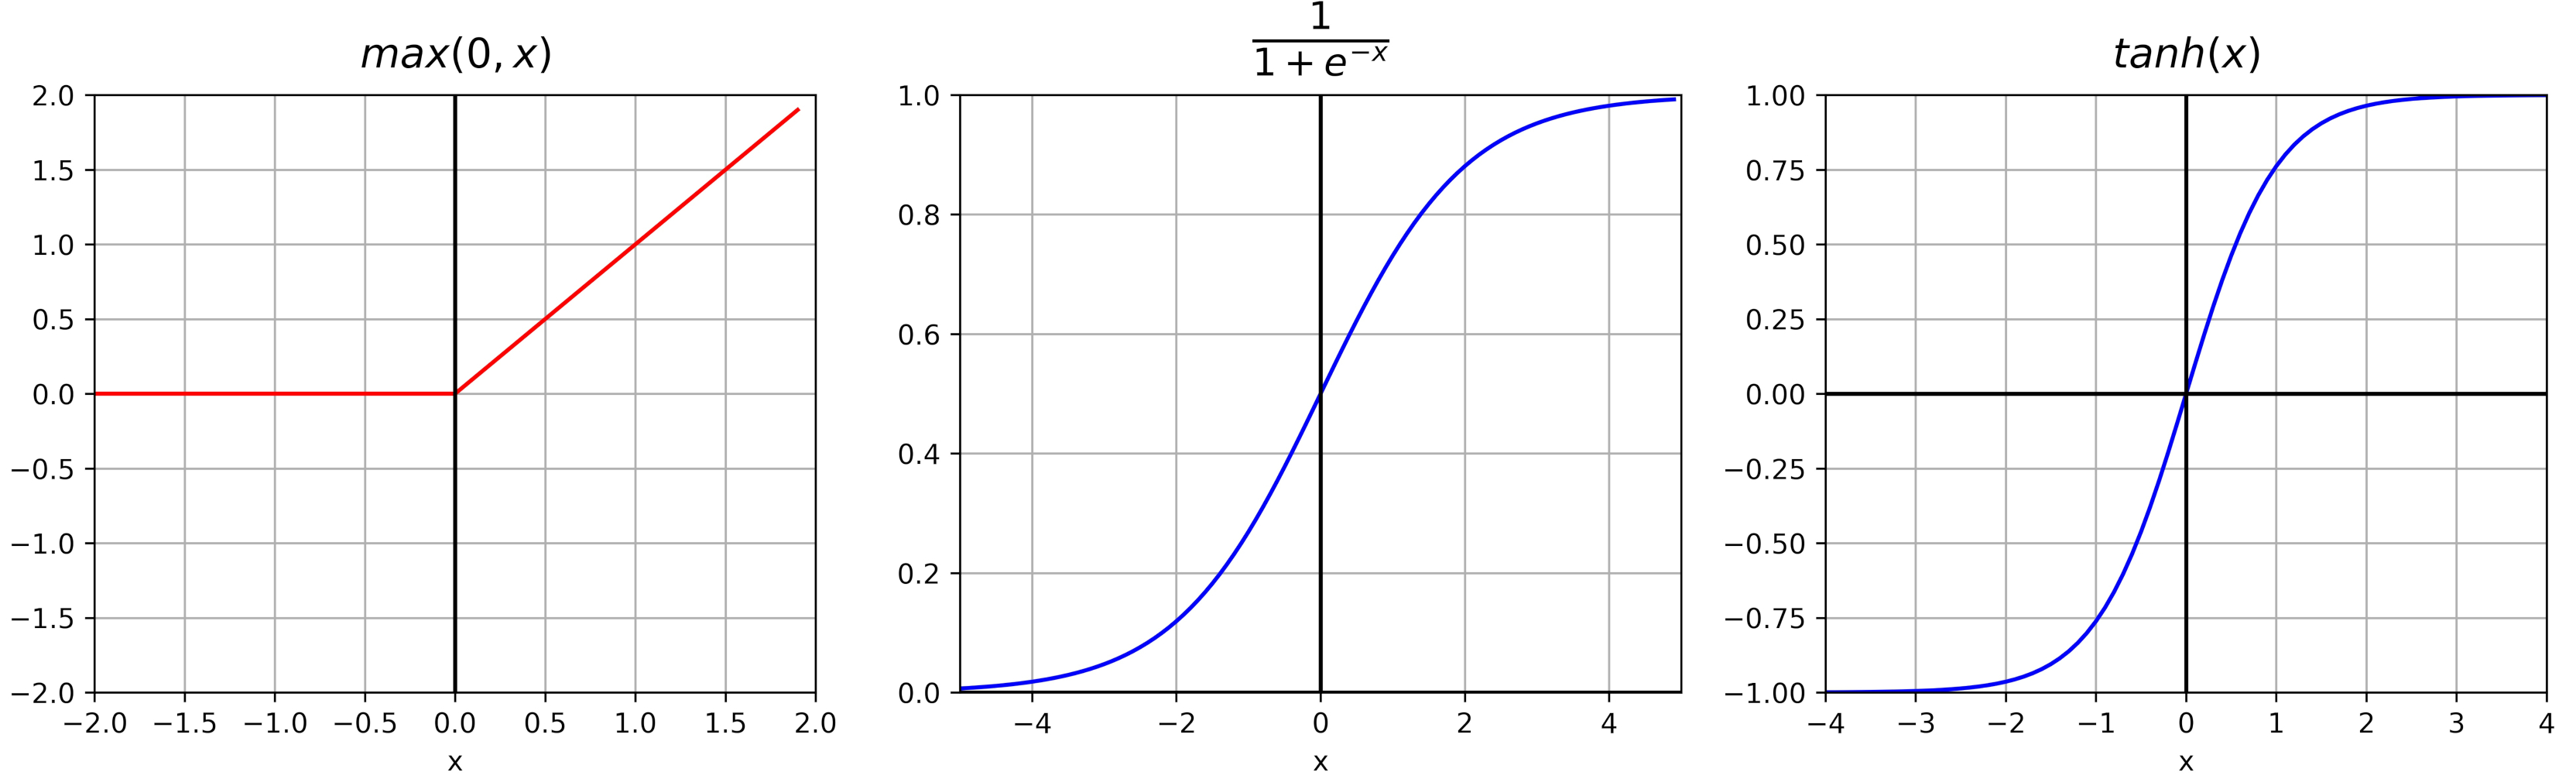
\includegraphics[width=\textwidth]{images/activationfunctions.jpg}
\end{frame}
%---------------------------
\begin{frame}{Correcting Errors}
\begin{enumerate}[1.]
    \item How do we drive our network's weights and biases towards the values that will give us the most correct predictions?
    \newline
    \item It makes sense to push the network's output as close to the desired output as possible via the minimization of some loss function $\mathcal{L}$
    \newline
    \item This allows us to 'back-propagate' the error of the output with respect to the loss function $\mathcal{L}$ to all other weights and biases in the network
    
\end{enumerate}
\end{frame}
%---------------------------
\begin{frame}{Backpropagation and Gradient Descent (Rumelhart et al. 1987)}
    \begin{enumerate}[1.]
        \item Backpropagation involves adjusting each weight and bias in the network respective to its contribution to the overall error $\mathcal{L}$
        \item Weights and biases from nodes with higher activations will contribute greater to the overall 'error' average
        $$\mathcal{L}(y,y')=\frac{1}{2m}\sum^m_{i=1}(y'-y)^2$$
        \item Weight and bias updates can be made by calculating the gradients of the loss function with respect to the parameters
        $$\mathbf{W^{[L]}}_{t+1}={W^{[L]}}_t-\eta\frac{\partial\mathcal{L}}{\partial W^{[L]}}_t=W^{[L]}-\eta\nabla_{\theta_w}\mathcal{L}$$
        $$\mathbf{b^{[L]}}_{t+1}=b^{[L]}_t-\eta\frac{\partial\mathcal{L}}{\partial b^{[L]}_t}=b^{[L]}_t-\eta\nabla_{\theta_b}\mathcal{L}$$
    \end{enumerate}
\end{frame}
%---------------------------
\begin{frame}{What does Gradient Descent Look Like?}
    \includegraphics[width=\textwidth]{images/gradientdescent.jpg}
\end{frame}
%---------------------------
\section{Other types of ANN}
\subsection{Convolutional Neural Networks}
%---------------------------
\begin{frame}{Convolutional Networks (CNNs)}
\begin{center}
    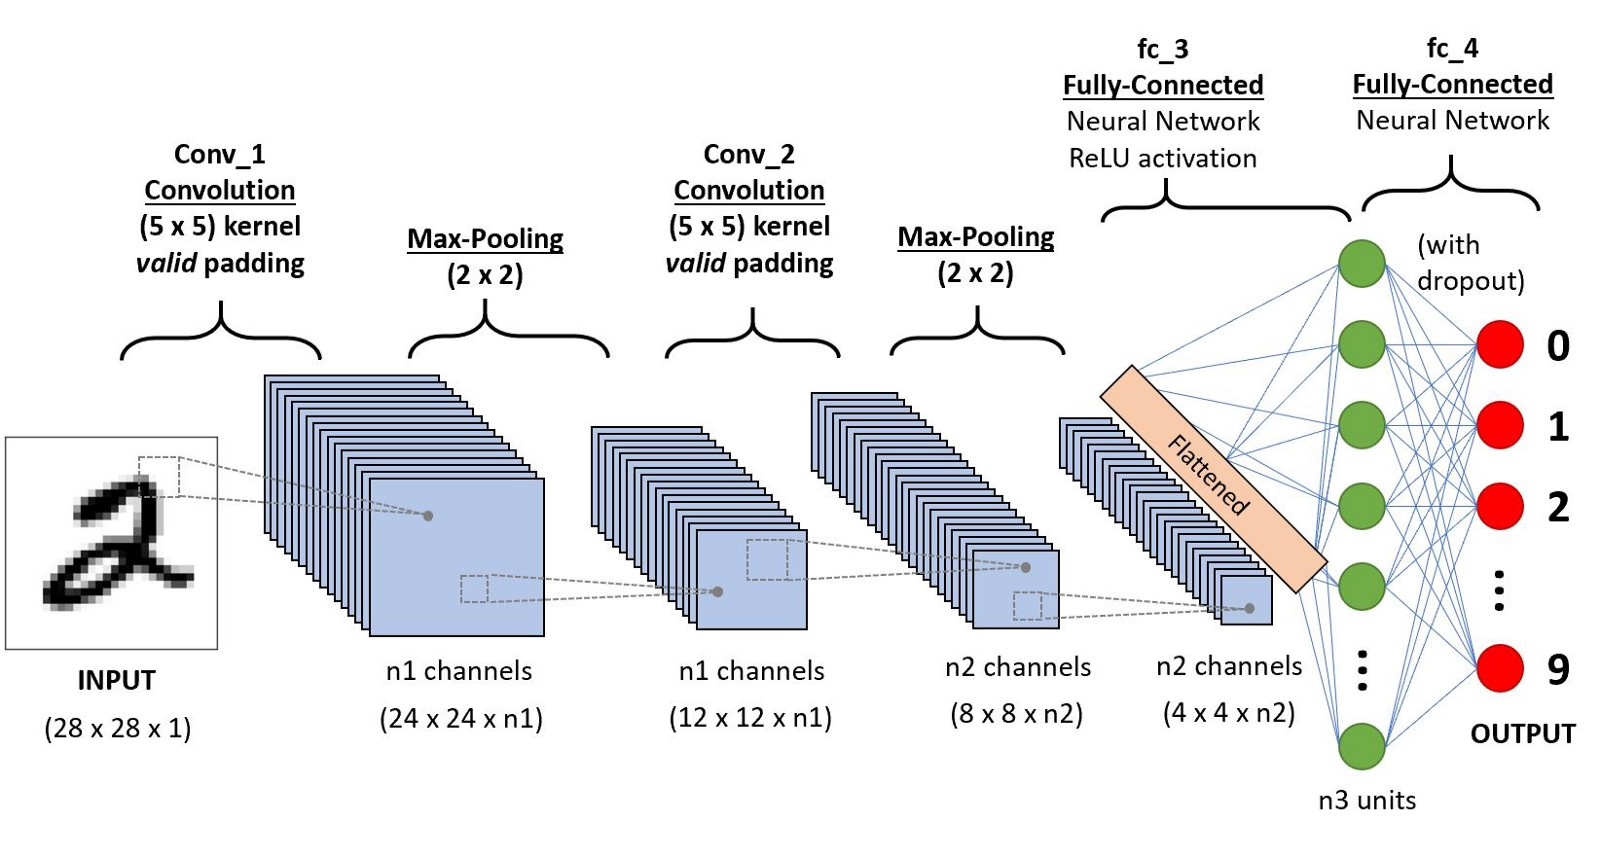
\includegraphics[width=\textwidth]{nets/alexnet.jpg}
\end{center}
\end{frame}
\begin{frame}{Why CNNs?}
    \centerline{\href{http://www.cs.cmu.edu/~aharley/vis/conv/flat.html}{Visualization (Harley 2017)}}
    \begin{enumerate}[1.]
        \item Inspired by visual 'receptive fields' - monkey visual cortexes contain neurons that individually respond to small 'regions' in the visual field (Hubel and Wiesel, 1968)
        \item Ex: Two different pictures of cats, while both pictures of cats, may trigger completely different groups of neurons
        \item CNNs use image kernels to capture complex patterns in different spatial arrangements of similar output classes
        \item The Kernel 'Formula'
        $$\displaystyle G[m,n]=(f\circ g)[m,n]=\sum_j\sum_kg[j,k]f[m-j,n-k]$$
    \end{enumerate}
\end{frame}
%---------------------------
%---------------------------
%---------------------------
%---------------------------
\begin{frame}{The Convolution Operation}
    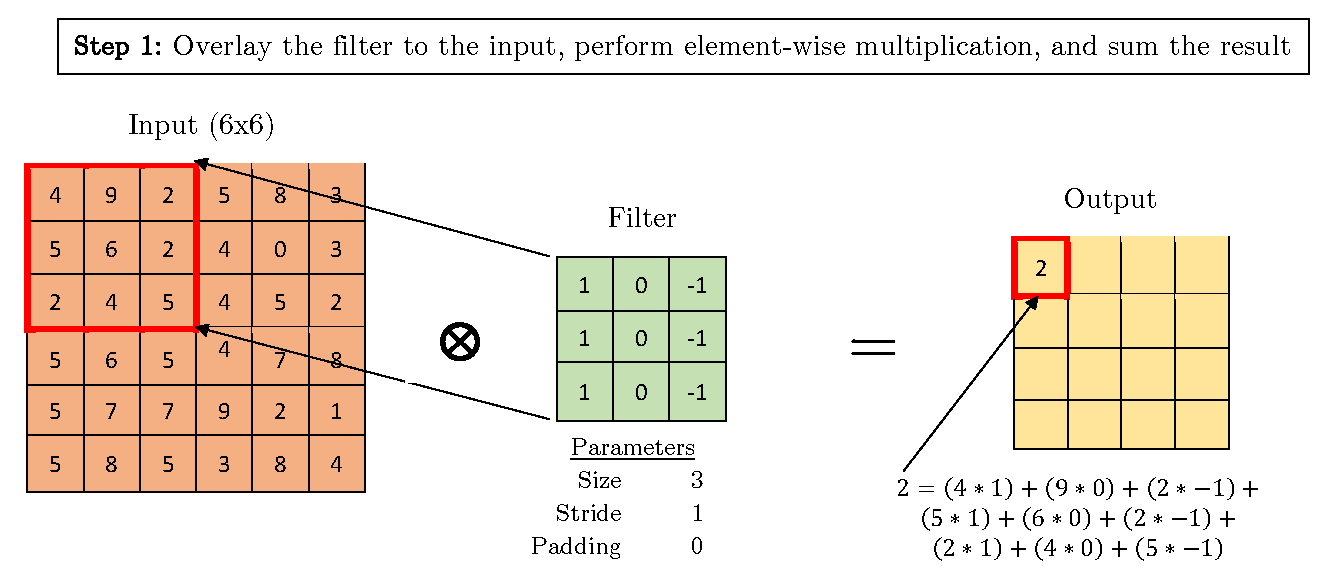
\includegraphics[width=\textwidth]{nets/conv/convstep1.pdf}
\end{frame}
%---------------------------
\begin{frame}{The Convolution Operation (Continued)}
    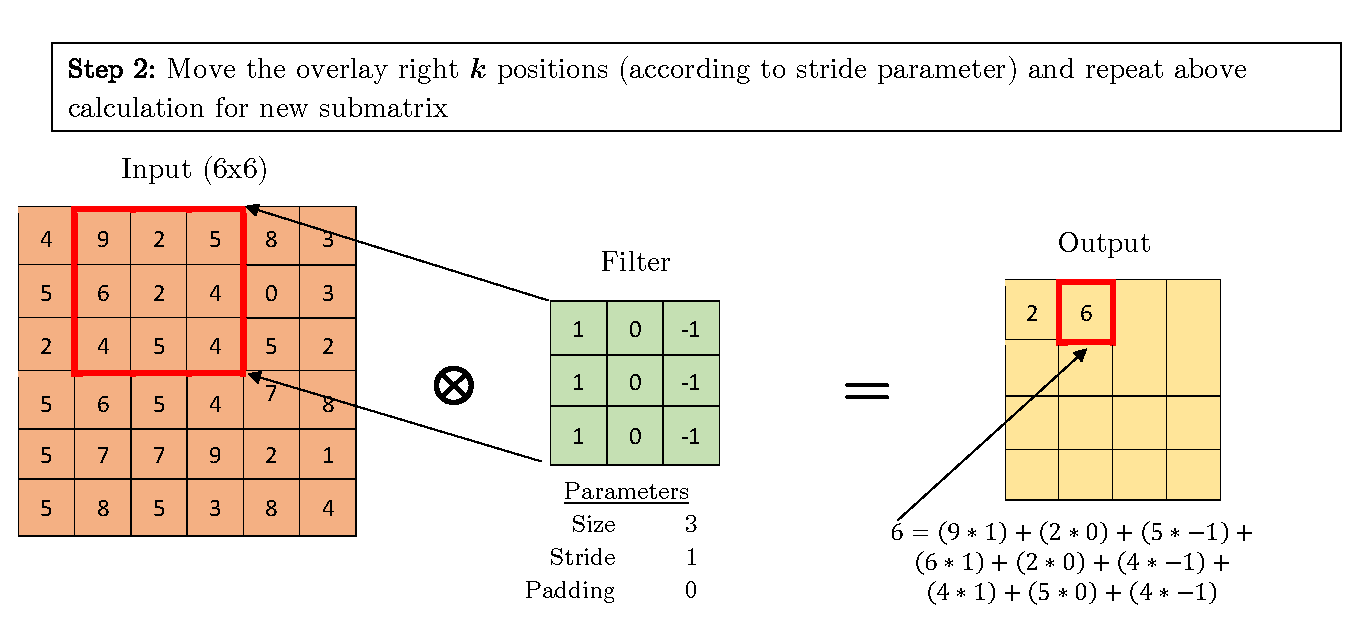
\includegraphics[width=\textwidth]{nets/conv/convstep2.pdf}
\end{frame}
%---------------------------
\begin{frame}{The Convolution Operation (Continued, Continued))}
\begin{center}
    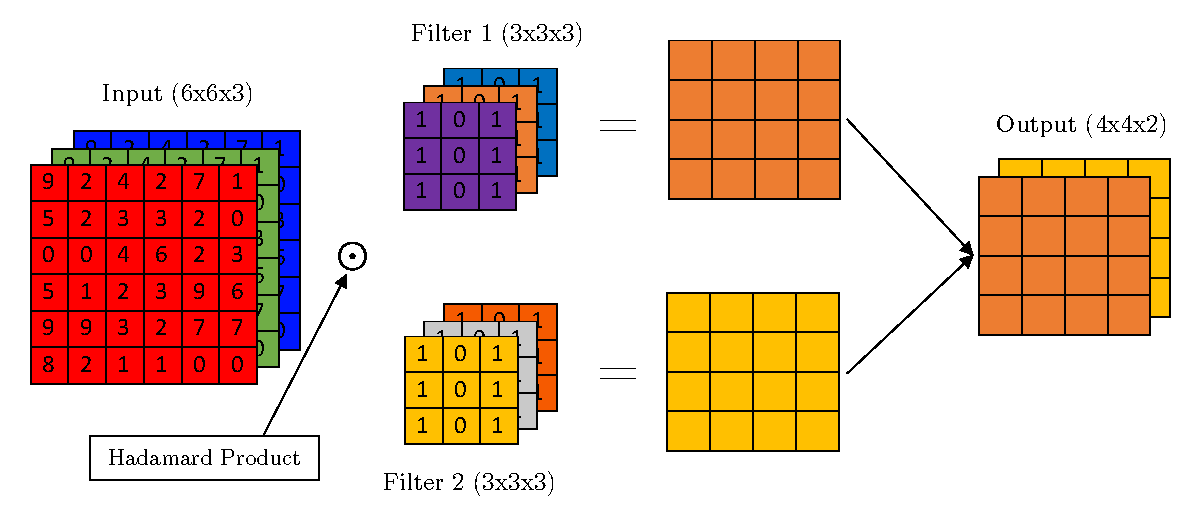
\includegraphics[width=\textwidth]{nets/convslide1.pdf}
\end{center}
\end{frame}
%---------------------------
\begin{frame}{What does that look like?}
    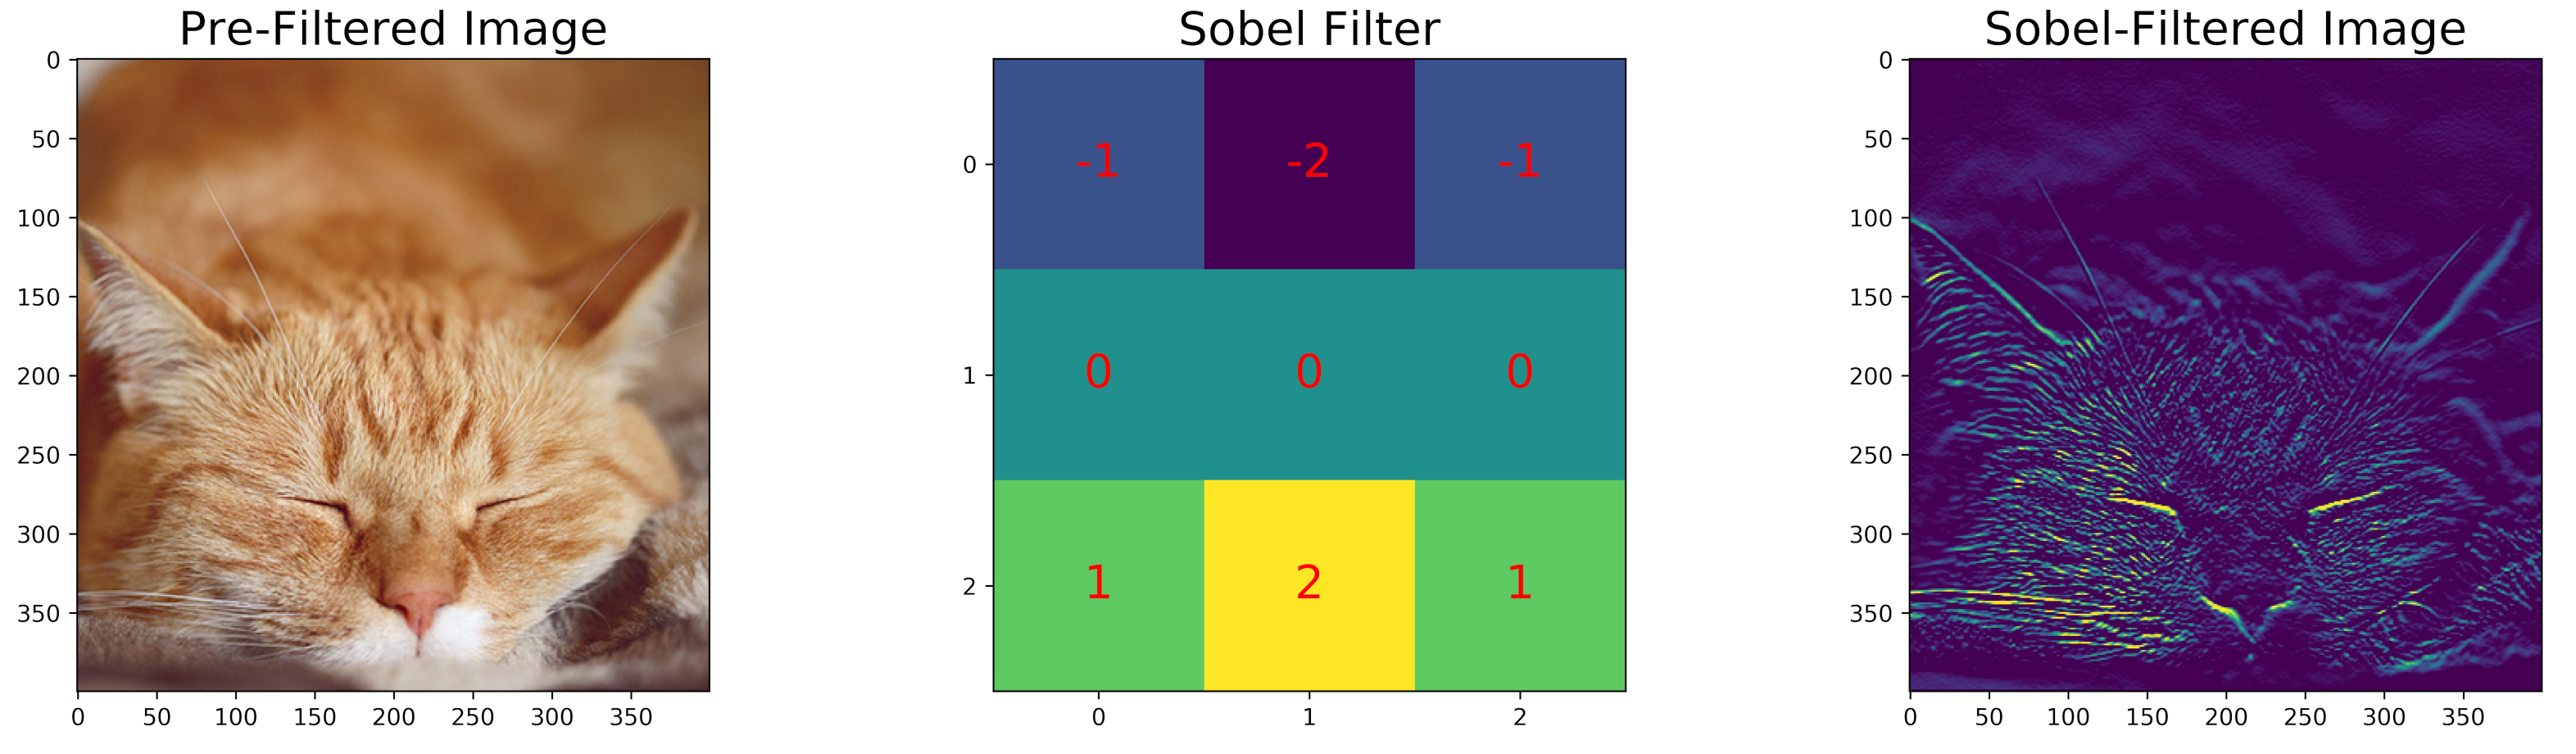
\includegraphics[width=\textwidth]{images/filterplots.jpg}\newline
\end{frame}
%---------------------------
\begin{frame}{Recurrent Neural Networks}
    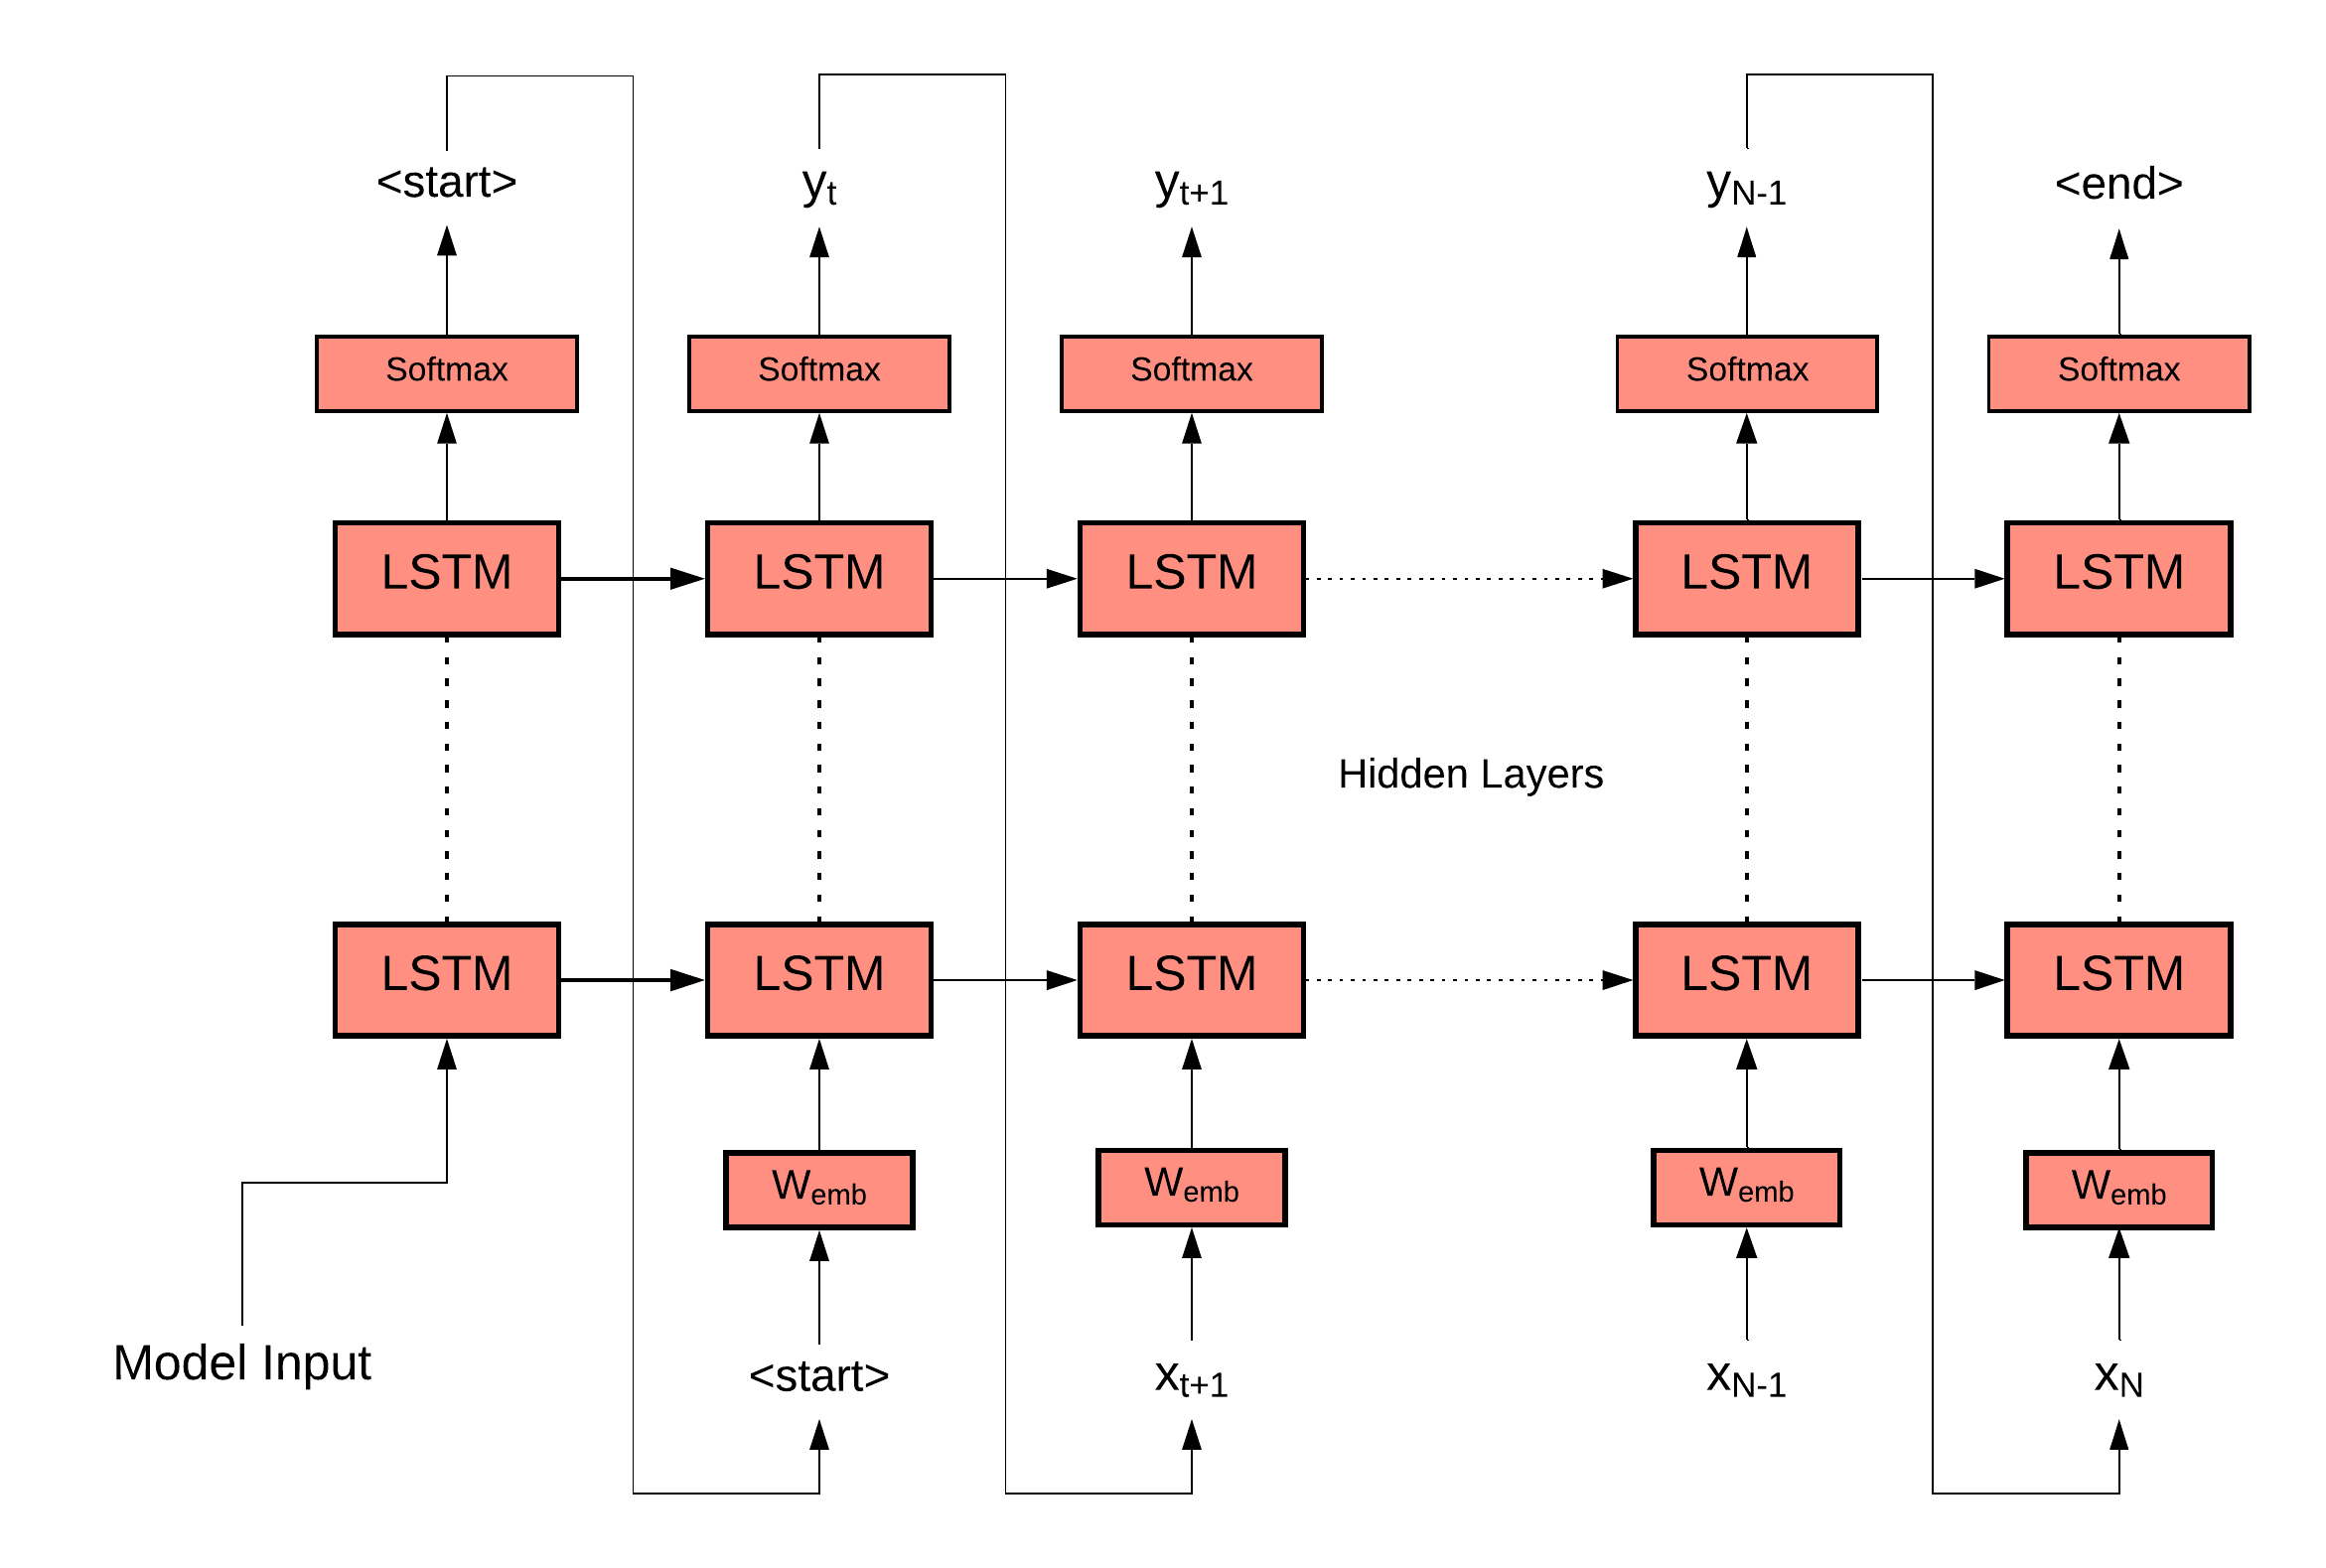
\includegraphics[scale=0.5]{nets/rnn.png}
\end{frame}
%---------------------------
\subsection{Recurrent Networks (RNN/LSTM)}
%---------------------------
\begin{frame}{Why Recurrent Networks?}
    \begin{enumerate}[1.]
        \item FCNNs and CNNs lack \textit{memory}
        \item Additionally, not all problems can be converted into ones with fixed-length inputs/outputs
        \begin{enumerate}[a.]
            \item Simple: Determine if a number is even. 1000010100 is even, 100011 is not
        \end{enumerate}
        \item RNNs were invented for this purpose; each neuron or 'unit' can maintain information about previous inputs with its internal memory
        \item Context matters; the structure of natural language, peptide \textbf{sequence}
        \item Additionally, RNNs can model sequences having variable length, and share weights across time steps; the amount of time an RNN keeps its intermediate values is not decided a priori
    \end{enumerate}
\end{frame}
%---------------------------
\begin{frame}{LSTM: Long Short-Term Memory}
\begin{center}
    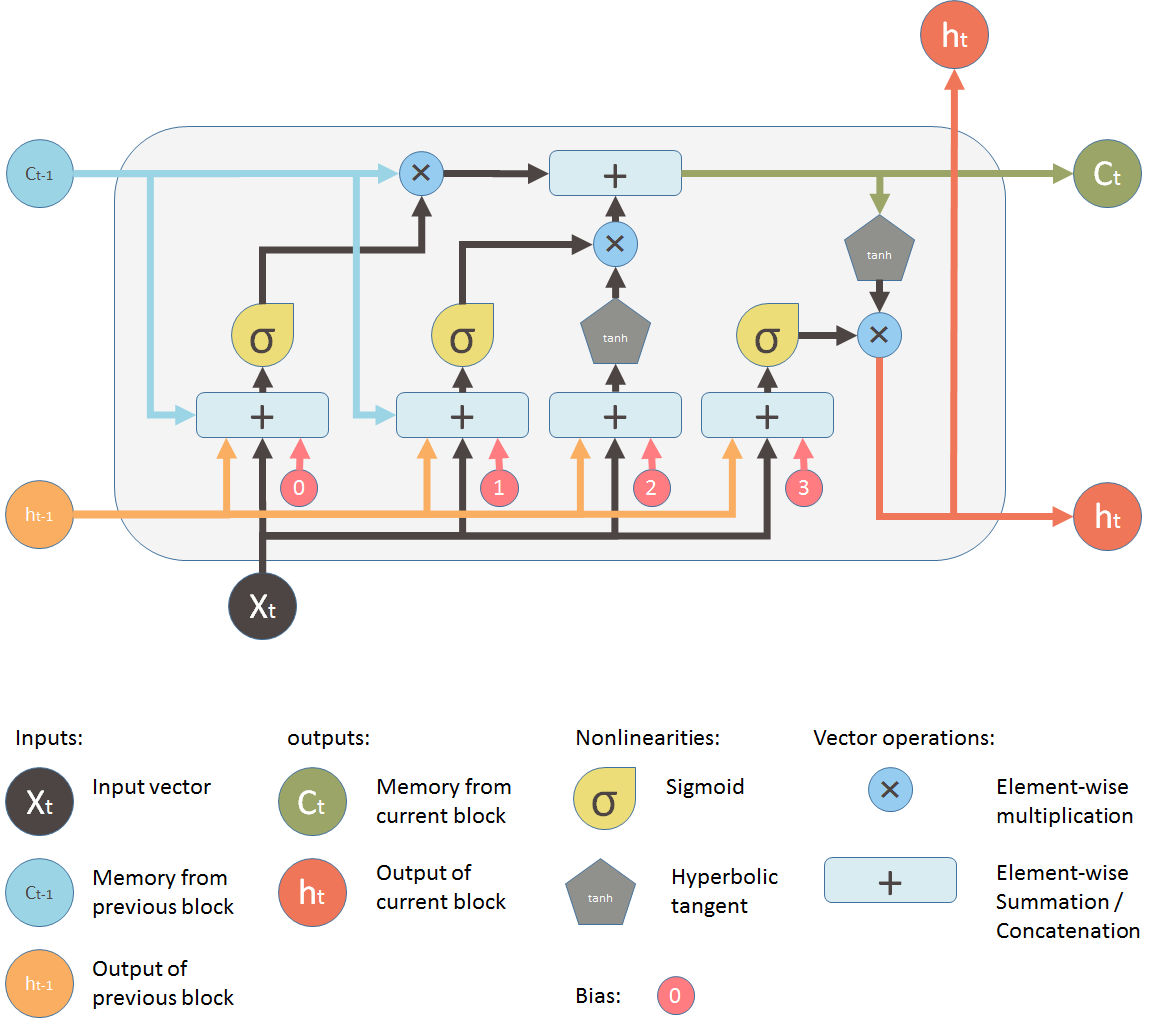
\includegraphics[height=0.75\textheight]{nets/lstm.png}
\end{center}
\end{frame}
%---------------------------
\begin{frame}{Forward Propagation in an RNN}
    \begin{algorithm}[H]
        \caption{Forward Propagation in an LSTM}
        \begin{algorithmic}[2]
        \Require
            \Statex Input Weights: $\mathbf{W}_z, \mathbf{W}_i, \mathbf{W}_f, \mathbf{W}_o \in\mathbb{R}^{M\times N}$
            \Statex Recurrent Weights: $\mathbf{R}_z, \mathbf{R}_i, \mathbf{R}_f, \mathbf{R}_o \in\mathbb{R}^{N\times N}$
            \Statex Peephole Weights: $\mathbf{p}_i, \mathbf{p}_f, \mathbf{p}_o \in\mathbb{R}^N$
            \Statex Bias Weights: $\mathbf{b}_z, \mathbf{b}_i, \mathbf{b}_f, \mathbf{b}_o \in\mathbb{R}^N$
        \Procedure{Forward Pass}{}
            \State $\mathbf{z}_t=g(\mathbf{W}_z\mathbf{x}_t+\mathbf{R}_z\mathbf{y}_{t-1})$ \Comment{Block Input}
            \State $\mathbf{i}_t=\sigma(\mathbf{W}_i\mathbf{x}_t+\mathbf{R}_i\mathbf{y}_{t-1}+\mathbf{p}_i\odot\mathbf{c}_{t-1}+\mathbf{b}_i)$ \Comment{Input Gate}
            \State $\mathbf{f}_t=\sigma(\mathbf{W}_f\mathbf{x}_t+\mathbf{R}_f\mathbf{y}_{t-1}+\mathbf{p}_f\odot\mathbf{c}_{t-1}+\mathbf{b}_f)$ \Comment{Forget Gate}
            \State $\mathbf{c}_t=\mathbf{z}_t\cdot\mathbf{i}_t+\mathbf{c}_{t-1}\cdot\mathbf{f}_t$ \Comment{Cell}
            \State $\mathbf{o}_t=\sigma(\mathbf{W}_o\mathbf{x}_t+\mathbf{R}_o\mathbf{y}_{t-1}+\mathbf{p}_o\odot\mathbf{c}_t+\mathbf{b}_o)$ \Comment{Output Gate}
            \State $\mathbf{y}_t=h(\mathbf{c}_t)\cdot\mathbf{o}_t$ \Comment{Block Output}
        \EndProcedure
    \end{algorithmic}
    \end{algorithm}
\end{frame}
%---------------------------
\begin{frame}{Different RNNs And Their Purposes}
    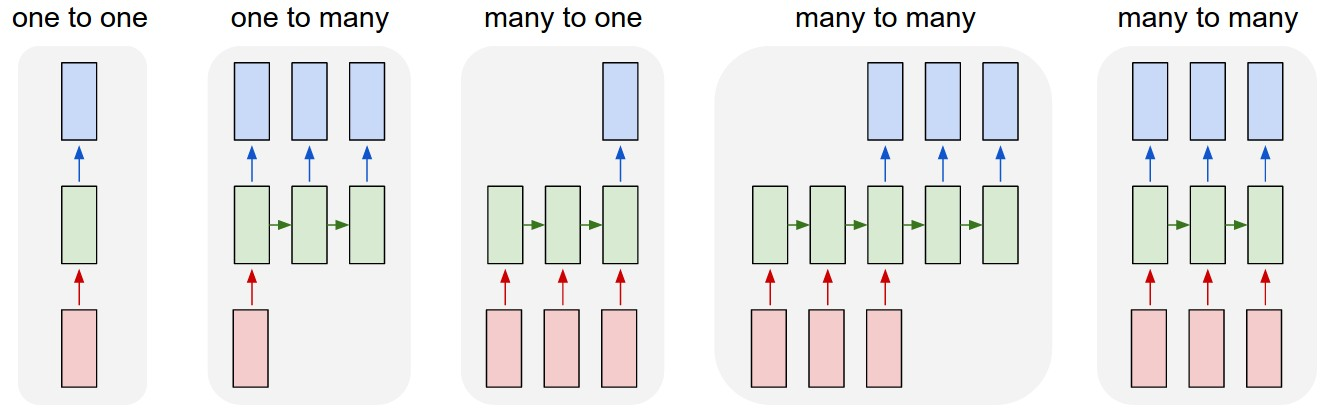
\includegraphics[width=\textwidth]{images/b4sus.jpg}
    \begin{enumerate}[i.]
        \item One-to-one: Vanilla FCNN
        \item One-to-many: Sequence Output (image captioning)
        \item Many-to-one: Sequence input (sentiment analysis)
        \item Many-to-many: Sequence input $\&$ output (machine translation)
        \item Many-to-many: Synced sequence input/output (video frame labeling)
    \end{enumerate}
\end{frame}
%---------------------------
%---------------------------
\section{Putting it All Together}
\subsection{The Image Captioning Problem}
%---------------------------
\begin{frame}{How does this help?}
    \begin{enumerate}[1.]
        \item Image Captioning: take some input image and output a natural language description 
        \item Finds uses in many different disciplines:
        \begin{enumerate}[a.]
            \item MRI Scans: Ground-truth can be time consuming and varies between physicians. Automated captioning of MRI scans allows for a speed up of this process (augmentation)
            \item Automated diagnosis: arrhythmia etc
            \item Image alternate text: People who are blind benefit from text descriptions of images commonly hard-coded in HTML 
        \end{enumerate}
        \item Current 'state of the art' involves some mix of RNN/CNN or some derivative network
    \end{enumerate}
\end{frame}
%---------------------------
%---------------------------
\begin{frame}{An Input Image $\rightarrow$ Caption}
    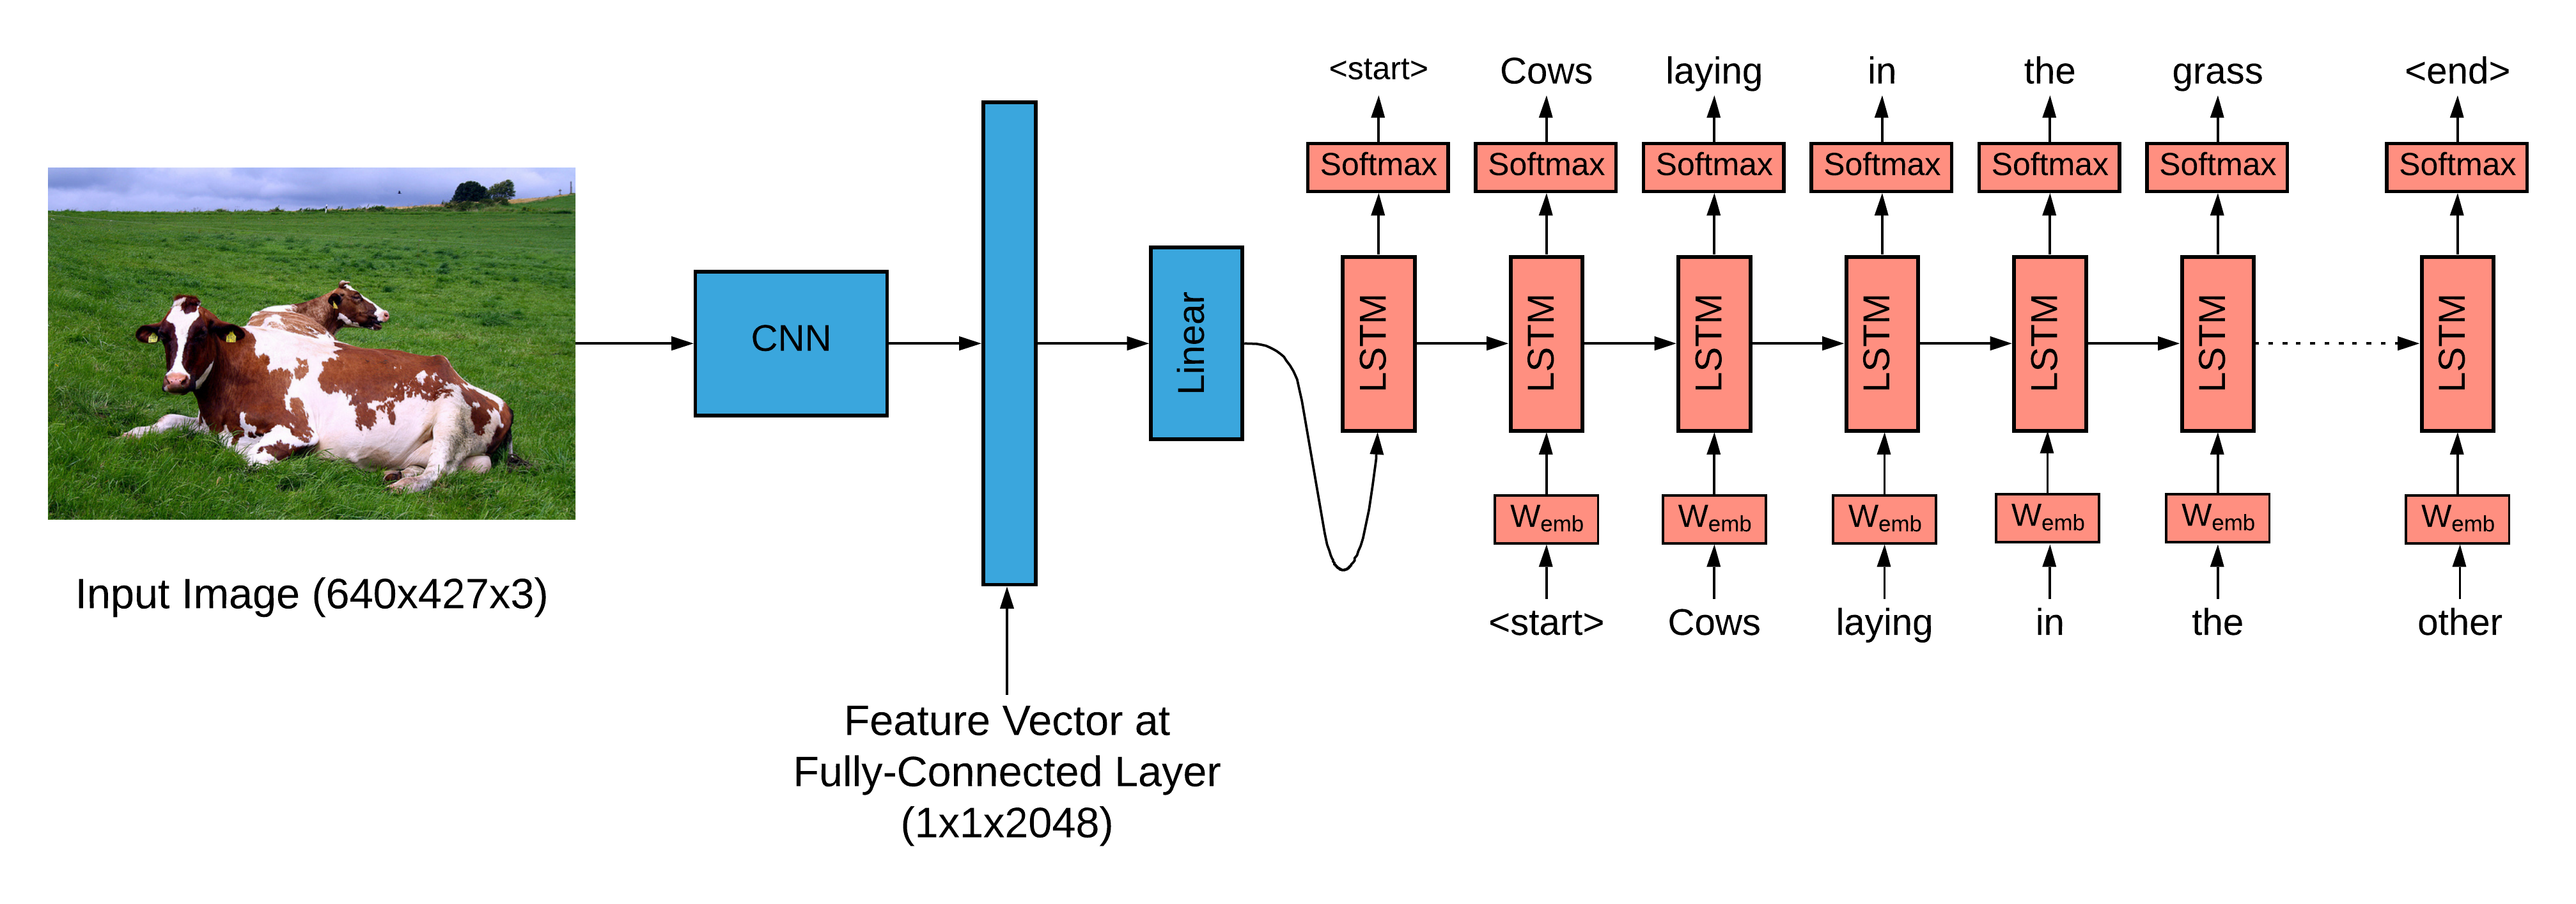
\includegraphics[width=\textwidth]{nets/conv/CNN-LSTM.png}
    \newline
    \centerline{\Large Caption: Cows laying in the grass}
\end{frame}
%---------------------------
%---------------------------
\begin{frame}{Other Types of Networks and 'AI'}
    \begin{enumerate}[1.]
        \item Generative Adversarial Networks (Goodfellow et al. 2014): Two networks (a generative network $G$ and a discriminative network $D$) play a specialized version of minimax:
    \end{enumerate}
    \centerline{$\displaystyle \argmin_G\argmax_DV(D,G)=\expected_{\textbf{x}\sim\textit{p}_{data}(\textbf{x})}[log(D(\textbf{x})]+\expected_{\textbf{z}\sim\textit{p}_{z}(\textbf{z})}[log(1-D(G(\textbf{z})))]$}
    \begin{enumerate}[2.]
        \item Deep Residual Networks (He et al. 2015): Optimize some network output $\mathcal{F}(x):=\mathcal{H}(x)+x$ where $\mathcal{H}(x)$ is the network output of the input $x$.
        \item Reinforcement Learning: Evaluative rather than instructive feedback; a Markov Decision Process in which the 'agent' interacts with the environment to maximize some sort of scalar reward. (\href{https://mitpress.mit.edu/books/reinforcement-learning-second-edition}{Sutton/Barto Book})
    \end{enumerate}
\end{frame}
%---------------------------
%---------------------------
\begin{frame}{Interested in Learning More?}
    \begin{enumerate}[1.]
        \item \textcolor{blue}{\href{https://cs230.stanford.edu/}{Stanford CS230: Deep Learning (Free!)}}
        \newline
        \item \textcolor{blue}{\href{https://www.coursera.org/specializations/deep-learning}{Coursera: Deep Learning Specialization}}
        \newline
        \item \textcolor{blue}{\href{http://neuralnetworksanddeeplearning.com/}{Michael Nielsen: Neural Networks and Deep Learning}}
        \newline
        \item \textcolor{blue}{\href{https://www.youtube.com/playlist?list=PLZHQObOWTQDNU6R1_67000Dx_ZCJB-3pi}{3Blue1Brown Youtube Series: Neural Networks}}
        \newline
        \item \textcolor{blue}{\href{https://github.com/lbmallory/NNPresentationCode}{Github}}
        \newline
        \item ....Books!
    \end{enumerate}
\end{frame}
%---------------------------
\begin{frame}{That's all!}
    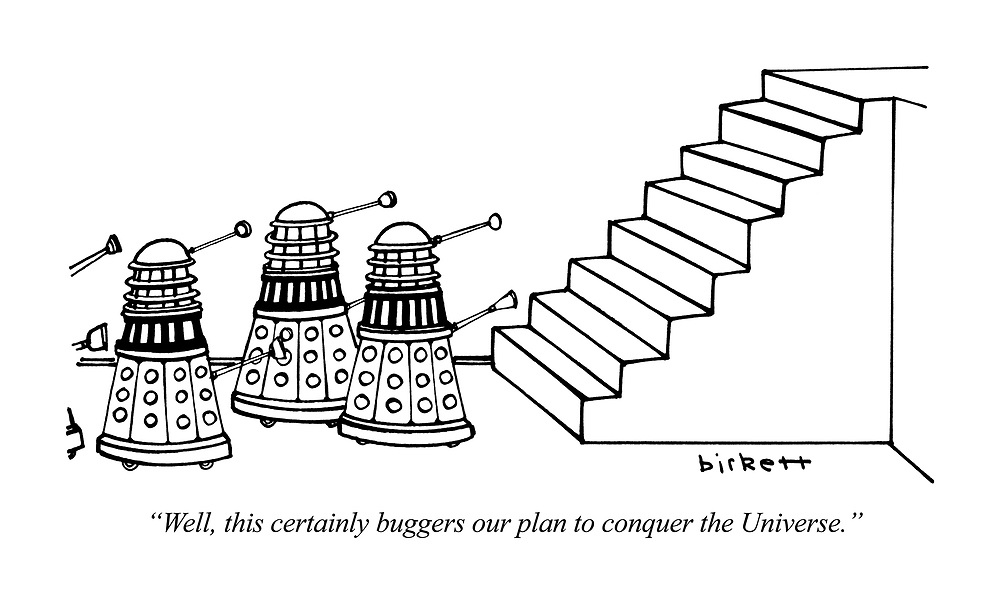
\includegraphics[height=0.75\textheight,width=\textwidth]{images/robots.jpg}
\end{frame}
%---------------------------
\end{document}
